\documentclass[a4paper]{book}
\usepackage[utf8]{vietnam}
\usepackage{csquotes}
\usepackage{lipsum}
\usepackage{times}
\usepackage[table,xcdraw]{xcolor}
\usepackage{multirow}
\usepackage[left=3cm,right=2cm,top=2cm,bottom=2.5cm]{geometry}
\setlength{\parindent}{4em}
\setlength{\parskip}{1em}
\setcounter{tocdepth}{5}
\setcounter{secnumdepth}{5}
\renewcommand{\baselinestretch}{1.5}
\usepackage{fancyhdr} 
\fancyhf{}
\cfoot{\thepage}
\pagestyle{fancy}    
\usepackage{graphicx}
\usepackage{caption}
\DeclareCaptionFormat{citation}{%
	\ifx\captioncitation\relax\relax\else
	\captioncitation\par
	\fi
	#1#2#3\par}
\newcommand*\setcaptioncitation[1]{\def\captioncitation{\textit{Source:}~#1}}
\let\captioncitation\relax
\captionsetup{format=citation,justification=centering}  
%\usepackage{wallpaper}
%\usepackage[firstpage]{draftwatermark} 
\usepackage{listings}
\usepackage{xcolor}
\definecolor{codegreen}{rgb}{0,0.6,0}
\definecolor{codegray}{rgb}{0.5,0.5,0.5}
\definecolor{codepurple}{rgb}{0.58,0,0.82}
\definecolor{backcolour}{rgb}{1,1,1}
\lstdefinestyle{mystyle}{
	backgroundcolor=\color{backcolour},   
	commentstyle=\color{codegreen},
	keywordstyle=\color{magenta},
	numberstyle=\tiny\color{codegray},
	stringstyle=\color{codepurple},
	basicstyle=\ttfamily\footnotesize,
	breakatwhitespace=false,         
	breaklines=true,                 
	captionpos=b,                    
	keepspaces=true,                 
	numbers=left,                    
	numbersep=5pt,                  
	showspaces=false,                
	showstringspaces=false,
	showtabs=false,                  
	tabsize=2
}
\lstset{style=mystyle}
\usepackage{tikz}
\usetikzlibrary{positioning}
\tikzstyle {round} = [circle, draw=green!60, fill=green!5, very thick, minimum size=7mm]
\tikzstyle {squared} = [rectangle, draw=red!60, fill=red!5, very thick, minimum size=5mm]
\tikzstyle {output} = [coordinate, node distance = 3cm]
\tikzstyle {textred} = [text=red] 
\usepackage{scrextend}
\changefontsizes{14pt}
%\usepackage{background}
\usetikzlibrary{calc}
%\backgroundsetup{scale = 1, angle = 0, opacity = 0.2,
%contents = {\includegraphics[width = 0.9\paperwidth,
%height = 0.9\paperheight, keepaspectratio] {hust.png}}}

%\backgroundsetup{scale = 1, angle = 0, opacity = 0.2,
%contents = {\includegraphics[width = 0.97\paperwidth,
%height = 0.97\paperheight, keepaspectratio] {bia.png}}}
\begin{document}
\begin{titlepage}
%\SetWatermarkText{\includegraphics[width = 0.97\paperwidth,
%height = 0.97\paperheight]{bia.png}}
%\SetWatermarkAngle{0} 
%\SetWatermarkText{\includegraphics[scale=1]{hust.png}}
%\SetWatermarkAngle{0}
\begin{tikzpicture}[remember picture,overlay,inner sep=0,outer sep=0]
     \draw[blue!70!black,line width=4pt] ([xshift=-1.5cm,yshift=-2cm]current page.north east) coordinate (A)--([xshift=1.5cm,yshift=-2cm]current page.north west) coordinate(B)--([xshift=1.5cm,yshift=2cm]current page.south west) coordinate (C)--([xshift=-1.5cm,yshift=2cm]current page.south east) coordinate(D)--cycle;

     \draw ([yshift=0.5cm,xshift=-0.5cm]A)-- ([yshift=0.5cm,xshift=0.5cm]B)--
     ([yshift=-0.5cm,xshift=0.5cm]B) --([yshift=-0.5cm,xshift=-0.5cm]B)--([yshift=0.5cm,xshift=-0.5cm]C)--([yshift=0.5cm,xshift=0.5cm]C)--([yshift=-0.5cm,xshift=0.5cm]C)-- ([yshift=-0.5cm,xshift=-0.5cm]D)--([yshift=0.5cm,xshift=-0.5cm]D)--([yshift=0.5cm,xshift=0.5cm]D)--([yshift=-0.5cm,xshift=0.5cm]A)--([yshift=-0.5cm,xshift=-0.5cm]A)--([yshift=0.5cm,xshift=-0.5cm]A);


     \draw ([yshift=-0.3cm,xshift=0.3cm]A)-- ([yshift=-0.3cm,xshift=-0.3cm]B)--
     ([yshift=0.3cm,xshift=-0.3cm]B) --([yshift=0.3cm,xshift=0.3cm]B)--([yshift=-0.3cm,xshift=0.3cm]C)--([yshift=-0.3cm,xshift=-0.3cm]C)--([yshift=0.3cm,xshift=-0.3cm]C)-- ([yshift=0.3cm,xshift=0.3cm]D)--([yshift=-0.3cm,xshift=0.3cm]D)--([yshift=-0.3cm,xshift=-0.3cm]D)--([yshift=0.3cm,xshift=-0.3cm]A)--([yshift=0.3cm,xshift=0.3cm]A)--([yshift=-0.3cm,xshift=0.3cm]A);

   \end{tikzpicture}
\begin{center}   
    \textbf{TRƯỜNG ĐẠI HỌC SƯ PHẠM KỸ THUẬT \\ THÀNH PHỐ HỒ CHÍ MINH}
    \textbf{\\KHOA CÔNG NGHỆ THÔNG TIN}
\end{center}
\begin{center}
	\renewcommand{\baselinestretch}{1.5}
    
\includegraphics[scale=0.6]{cntt.jpg}
    
    \vspace{10pt}
    \fontsize{18pt}{17pt}\selectfont 
    \textbf{BÁO CÁO}
    \vspace{7pt}
    \textbf{QUẢN LÝ DỰ ÁN}
\end{center}
\begin{flushleft}
    \fontsize{14pt}{17pt}\selectfont  
    \textbf{\textsl{ĐỀ TÀI}}
\end{flushleft}
\begin{center}
    \fontsize{18pt}{17pt}\selectfont
    \textbf{XÂY DỰNG WEBSITE XEM PHIM TRỰC TUYẾN \\}
    \textbf{VÀ DỊCH VỤ HOSTING}
\end{center}
\textbf{GV hướng dẫn: Thầy Hoàng Long}
\\
\textbf{Nhóm sinh viên thực hiện:}
\begin{tabbing}
\hspace{8cm}\=\hspace{3cm}\=\hspace{3cm} \kill
{\it \textbf{Họ và tên}}\>{\it \textbf{MSSV}}\>{\it \textbf{Mã lớp}}\\
\begin{bfseries}Lâm Thế Vinh\end{bfseries}\> \begin{bfseries}16110523\end{bfseries}\> \begin{bfseries}1611IS\end{bfseries}\\
\begin{bfseries}Trần Phát Hưng\end{bfseries}\> \begin{bfseries}16110350\end{bfseries}\> \begin{bfseries}1611IS\end{bfseries}\\
\begin{bfseries}Nguyễn Bá Thuận\end{bfseries}\> \begin{bfseries}16110350\end{bfseries}\> \begin{bfseries}1611IS\end{bfseries}\\

\end{tabbing}
\begin{center}
    \textbf{Hồ Chí Minh, 2019}
\end{center}
\vspace{10pt}
\end{titlepage}
\tableofcontents
\chapter*{Lời mở đầu}
\chapter{Giới thiệu khách hàng}
Phía khách hàng là người cũng có hiểu biết về kiến thức công nghệ thông tin, đưa ra các yêu cầu về thiết kế, chức năng, nền tảng áp dụng cho dự án "Xây dựng website trực tuyến". Chi tiết yêu cầu được trình bày bên dưới.
\chapter{Yêu cầu khách hàng}
\section{Sơ đồ website}
Sơ đồ website cho biết website bao gồm những site nào, phân cấp ra sao.\\ \\
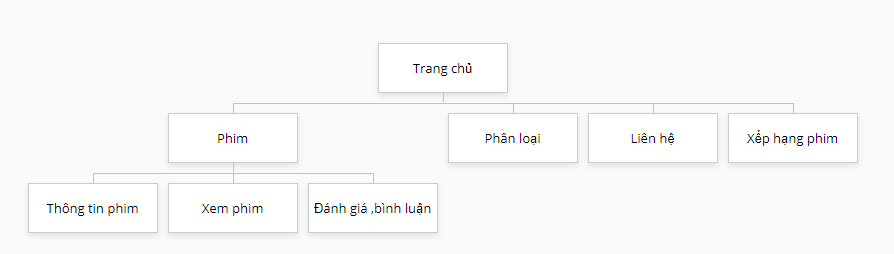
\includegraphics[scale=0.6]{sodo_website.PNG}
\section{Nội dung}
Nội dung mà phía khách hàng hướng tới là dữ liệu về phim. Trong đó phim bao gồm các thuộc tính sau: tên phim, năm sản xuất, thể loại, tóm tắt, trạng thái, quốc gia, thời lượng, ngôn ngữ, nhà sản xuất, đạo diễn, diễn viên, đánh giá.
\section{Thiết kế}
Khách hàng đưa ra các yêu cầu thiết kế sau:
\begin{itemize}
	\item Màu sắc: màu đen là màu chủ đạo
	\item Font: Open sans, sans-serif
	\item Thương hiệu: Phim hay
	\item Hỗ trợ hiển thị đa thiết bị (Responsive)
	\item Một số website có thể tham khảo: phimmoi.net, dongphim.net
\end{itemize}
\section{Chức năng}
- Số server hỗ trợ cho xem phim: 2 server\\
- Người dùng đăng nhập qua facebook để bình luận cho phim \\
- Tích hợp phân tích, theo dõi thói quen người dùng để đề xuất phim phù hợp \\
-  Tìm kiếm phim qua các thông tin: tên phim, đạo diễn, diễn viên, thể loại, năm sản xuất
\section{Nền tảng}
- Nền tảng được sử dụng cho dự án:
\begin{itemize}
	\item Client: single page(giao diện) reactjs hoặc vuejs , html, css, jquery
	\item Server: nodejs hoặc golang(server)
	\item Database: MongoDB, SQL server
\end{itemize}
\section{Hosting and Domain}
- Hosting được đặt tại Việt Nam\\
- Domain: phimhay.net\\
- Số lượng user có thể truy cập tối đa cùng lúc: 5000\\
\section{Yêu cầu bổ sung}
- Hướng dẫn chi tiết cách sử dụng sản phẩm cho người dùng\\
- Hệ thống phải có thời gian đáp ứng nhanh, thời gian phục hồi hệ thống khi có sự cố, thời gian phục vụ của hệ thống\\
- Phải có tính bảo mật và an toàn cao, chỉ những người có trách nhiệm trong nghiệp vụ mới được truy cập và sửa chữa\\
- Giải đáp mọi thắc mắc của khách hàng trong thời gian nhanh nhất (trong vòng 24 tiếng)\\
- Lắp đặt và bảo trì miễn phí trong 1 năm kể từ ngày hệ thống đi vào hoạt động.( Không yêu cầu thêm tính năng)\\
- Sao lưu và phục hồi dữ liệu: chức năng hỗ trợ thêm nếu tổ chức không có hệ thống máy chủ và nhân lực phục vụ cho việc sao lưu dữ liệu định kỳ
\chapter{Work Breakdown Structure (WBS)}
Dự án hiện tại được chia ra hai \textit{deliverable} đó là xây dựng \textit{website} xem phim trực tuyến và dịch vụ \textit{hosting}.
\section{Xây dựng website}
Là một trong hai \textit{deliverable} chính của dự án. Xây dựng \textit{website} được chia thành nhiều giai đoạn, mỗi giai đoạn sẽ có những \textit{sub-deliverable} hoặc \textit{work package} tương ứng.
\subsection{Lấy yêu cầu khách hàng}
Là giai đoạn đầu tiên trong xây dựng \textit{website} được xác định với một \textit{work package}. \textit{Work package 1}: Lấy yêu cầu khách hàng. Mục tiêu chính của gói công việc này là có được bảng đặc tả những yêu cầu của khách hàng về website của họ. Các yêu cầu về cách tổ chức website, cấu trúc trang, yêu cầu giao diện, yêu cầu chức năng,...\textit{Work package 1}: Lấy yêu cầu của khách hàng được miêu tả cụ thể trong bảng \ref{table:lay_yeu_cau}
\begin{table}[h!]
	\begin{center}
		\begin{tabular}{|p{4cm}|p{10cm}|}
			\hline
			\multicolumn{2}{|c|}{\cellcolor[HTML]{363636}{\color[HTML]{FFFFFF}Work package 1: Lấy yêu cầu khách hàng}}\\
			\hline
			\multirow{3}{*}{WP1. Objective} & $\bullet$ Đặc tả yêu cầu trang Front-end\\
			 & $\bullet$ Đặc tả yêu cầu trang Back-end \\
			 & $\bullet$ Đặc tả yêu cầu bảo mật	\\
			\hline
			\multirow{3}{*}{WP1. Description} & $\bullet$ Lấy yêu cầu của khách hàng về trang Front-end: giao diện (trang chủ, trang xem phim, trang tìm kiếm, trang chi tiết phim, trang khác nếu có), chức năng (xem phim, tìm kiếm, đăng nhập, bình luận, theo dõi thói quen, chức năng khác nếu có) \\
			& $\bullet$ Lấy yêu cầu khách hàng về trang Back-end: giao diện(trang quản trị phim, quản trị quản lý, trang khác nếu có), chức năng (quản trị phim, quản trị quản lý, chức năng khác nếu có)\\
			& $\bullet$ Lấy yêu cầu của khách hàng về bảo mật: phân quyền, sao lưu và phục hồi.\\
			\hline
		\end{tabular}
	\caption{Work Package 1: Lấy yêu cầu khách hàng}
	\label{table:lay_yeu_cau}
	\end{center}
\end{table}
\subsection{Phân tích và thiết kế}
Phân tích, thiết kế là giai đoạn thứ hai trong quy trình xây dựng \textit{website}. Trong giai đoạn này có 3 công việc chính cần làm là phân tích thiết kế cho Front-end site, Back-end site và cho các yêu cầu bảo mật.
\subsubsection{Phân tích, thiết kế Front-end site}
Trong phân tích và thiết kế cho \textit{Front-end site}, cần phân tích và thiết kế về mặt giao diện và chức năng.
\paragraph{Phân tích, thiết kế giao diện}
Phân tích và thiết kế giao diện theo yêu cầu của khách hàng. Mỗi trang trên giao diện sẽ được phân thành những \textit{work package} và được cụ thể hóa bằng các bảng tương ứng trong từng phần sau. Phân tích, thiết kế cho sự tương thích của giao diện cũng được chia thành work package.
\subparagraph{Phân tích, thiết kế giao diện trang chủ}Miêu tả cụ thể ở bảng \ref{table:front_end_thietke_trangchu}
\begin{table}[h!]
	\begin{center}
		\begin{tabular}{|p{4cm}|p{10cm}|}
			\hline
			\multicolumn{2}{|c|}{\cellcolor[HTML]{363636}{\color[HTML]{FFFFFF}Work package 2: Phân tích, thiết kế giao diện trang chủ}}\\
			\hline
			\multirow{1}{*}{WP2. Objective} & $\bullet$ Bảng thiết kế giao diện trang chủ\\
			\hline
			\multirow{2}{*}{WP2. Description} & $\bullet$ Phân tích phong cách, yêu cầu về giao diện trang chủ của khách hàng \\
			& $\bullet$ Thiết kế giao diện trang chủ theo yêu cầu của khách hàng\\
			\hline
		\end{tabular}
		\caption{Work Package 2: Phân tích, thiết kế giao diện trang chủ}
		\label{table:front_end_thietke_trangchu}
	\end{center}
\end{table}
\subparagraph{Phân tích, thiết kế giao diện trang xem phim}Miêu tả cụ thể ở bảng \ref{table:frontend_thietke_trangxemphim}
\begin{table}[h!]
	\begin{center}
		\begin{tabular}{|p{4cm}|p{10cm}|}
			\hline
			\multicolumn{2}{|c|}{\cellcolor[HTML]{363636}{\color[HTML]{FFFFFF}Work package 3: Phân tích, thiết kế giao diện trang xem phim}}\\
			\hline
			\multirow{1}{*}{WP3. Objective} & $\bullet$ Bảng thiết kế giao diện trang xem phim\\
			\hline
			\multirow{2}{*}{WP3. Description} & $\bullet$ Phân tích phong cách, yêu cầu về giao diện trang xem phim của khách hàng \\
			& $\bullet$ Thiết kế giao diện trang xem phim theo yêu cầu của khách hàng\\
			\hline
		\end{tabular}
		\caption{Work Package 3: Phân tích, thiết kế giao diện trang xem phim}
		\label{table:frontend_thietke_trangxemphim}
	\end{center}
\end{table}
\subparagraph{Phân tích, thiết kế giao diện trang tìm kiếm} Miêu tả cụ thể ở bảng \ref{table:frontend_thietke_trangtimkiem}
\begin{table}[h!]
	\begin{center}
		\begin{tabular}{|p{4cm}|p{10cm}|}
			\hline
			\multicolumn{2}{|c|}{\cellcolor[HTML]{363636}{\color[HTML]{FFFFFF}Work package 4: Phân tích, thiết kế giao diện trang tìm kiếm}}\\
			\hline
			\multirow{1}{*}{WP4. Objective} & $\bullet$ Bảng thiết kế giao diện trang tìm kiếm\\
			\hline
			\multirow{2}{*}{WP4. Description} & $\bullet$ Phân tích phong cách, yêu cầu về giao diện trang tìm kiếm của khách hàng \\
			& $\bullet$ Thiết kế giao diện trang tìm kiếm theo yêu cầu của khách hàng\\
			\hline
		\end{tabular}
		\caption{Work Package 3: Phân tích, thiết kế giao diện trang tìm kiếm}
		\label{table:frontend_thietke_trangtimkiem}
	\end{center}
\end{table}
\subparagraph{Phân tích, thiết kế giao diện trang chi tiết phim} Miêu tả cụ thể ở bảng \ref{table:frontend_thietke_trangchitietphim}
\begin{table}[h!]
	\begin{center}
		\begin{tabular}{|p{4cm}|p{10cm}|}
			\hline
			\multicolumn{2}{|c|}{\cellcolor[HTML]{363636}{\color[HTML]{FFFFFF}Work package 5: Phân tích, thiết kế giao diện trang chi tiết phim}}\\
			\hline
			\multirow{1}{*}{WP5. Objective} & $\bullet$ Bảng thiết kế giao diện trang chi tiết phim\\
			\hline
			\multirow{2}{*}{WP5. Description} & $\bullet$ Phân tích phong cách, yêu cầu về giao diện trang chi tiết phim của khách hàng \\
			& $\bullet$ Thiết kế giao diện trang chi tiết phim theo yêu cầu của khách hàng\\
			\hline
		\end{tabular}
		\caption{Work Package 5: Phân tích, thiết kế giao diện trang chi tiết phim}
		\label{table:frontend_thietke_trangchitietphim}
	\end{center}
\end{table}
\subparagraph{Phân tích, thiết kế tương thích giao diện} Miêu tả cụ thể ở bảng \ref{table:frontend_thietke_tuongthich}
\begin{table}[h!]
	\begin{center}
		\begin{tabular}{|p{4cm}|p{10cm}|}
			\hline
			\multicolumn{2}{|c|}{\cellcolor[HTML]{363636}{\color[HTML]{FFFFFF}Work package 6: Phân tích, thiết kế tương thích giao diện}}\\
			\hline
			\multirow{1}{*}{WP6. Objective} & $\bullet$ Bảng thiết kế giao diện trên smartphone (trang chủ, trang xem phim, trang chi tiết phim, trang tìm kiếm)\\
			\hline
			\multirow{2}{*}{WP6. Description} & $\bullet$ Phân tích yêu cầu khách hàng về giao diện trên smartphone \\
			& $\bullet$ Thiết kế giao diện trên smartphone theo yêu cầu của khách hàng\\
			\hline
		\end{tabular}
		\caption{Work Package 6: Phân tích, thiết kế tương thích giao diện}
		\label{table:frontend_thietke_tuongthich}
	\end{center}
\end{table}
\paragraph{Phân tích, thiết kế chức năng} Phân tích, thiết kế chức năng cho Front-end site theo yêu cầu của khách hàng. Mỗi chức năng được chia thành một \textit{work package} và có một bảng mô tả tương ứng.
\subparagraph{Phân tích, thiết kế chức năng xem phim} Miêu tả cụ thể ở bảng \ref{table:frontend_thietke_chucnang_xemphim}
\begin{table}[h!]
	\begin{center}
		\begin{tabular}{|p{4cm}|p{10cm}|}
			\hline
			\multicolumn{2}{|c|}{\cellcolor[HTML]{363636}{\color[HTML]{FFFFFF}Work package 7: Phân tích, thiết kế chức năng xem phim}}\\
			\hline
			\multirow{1}{*}{WP7. Objective} & $\bullet$ Bảng mô tả chức năng xem phim\\
			\hline
			\multirow{2}{*}{WP7. Description} & $\bullet$ Phân tích yêu cầu về chức năng xem phim của khách hàng \\
			& $\bullet$ Thiết kế chức năng xem phim theo yêu cầu của khách hàng\\
			\hline
		\end{tabular}
		\caption{Work Package 7: Phân tích, thiết kế chức năng xem phim}
		\label{table:frontend_thietke_chucnang_xemphim}
	\end{center}
\end{table}
\subparagraph{Phân tích, thiết kế chức năng tìm kiếm} Mô tả cụ thể ở bảng \ref{table:frontend_thietke_chucnang_timkiem}
\begin{table}[h!]
	\begin{center}
		\begin{tabular}{|p{4cm}|p{10cm}|}
			\hline
			\multicolumn{2}{|c|}{\cellcolor[HTML]{363636}{\color[HTML]{FFFFFF}Work package 8: Phân tích, thiết kế chức năng tìm kiếm}}\\
			\hline
			\multirow{1}{*}{WP8. Objective} & $\bullet$ Bảng mô tả chức năng tìm kiếm\\
			\hline
			\multirow{2}{*}{WP8. Description} & $\bullet$ Phân tích yêu cầu về chức năng tìm kiếm của khách hàng \\
			& $\bullet$ Thiết kế chức năng tìm kiếm theo yêu cầu của khách hàng\\
			\hline
		\end{tabular}
		\caption{Work Package 8: Phân tích, thiết kế chức năng tìm kiếm}
		\label{table:frontend_thietke_chucnang_timkiem}
	\end{center}
\end{table}
\subparagraph{Phân tích, thiết kế chức năng đăng nhập} Miêu tả cụ thể ở bảng \ref{table:frontend_thietke_chucnang_dangnhap}
\begin{table}[h!]
	\begin{center}
		\begin{tabular}{|p{4cm}|p{10cm}|}
			\hline
			\multicolumn{2}{|c|}{\cellcolor[HTML]{363636}{\color[HTML]{FFFFFF}Work package 9: Phân tích, thiết kế chức năng đăng nhập}}\\
			\hline
			\multirow{1}{*}{WP9. Objective} & $\bullet$ Bảng mô tả chức năng đăng nhập\\
			\hline
			\multirow{2}{*}{WP9. Description} & $\bullet$ Phân tích yêu cầu về chức năng đăng nhập của khách hàng \\
			& $\bullet$ Thiết kế chức năng đăng nhập theo yêu cầu của khách hàng\\
			\hline
		\end{tabular}
		\caption{Work Package 9: Phân tích, thiết kế chức năng đăng nhập}
		\label{table:frontend_thietke_chucnang_dangnhap}
	\end{center}
\end{table}
\subparagraph{Phân tích, thiết kế chức năng bình luận} Miêu tả cụ thể ở bảng \ref{table:frontend_thietke_chucnang_binhluan}
\begin{table}[h!]
	\begin{center}
		\begin{tabular}{|p{4cm}|p{10cm}|}
			\hline
			\multicolumn{2}{|c|}{\cellcolor[HTML]{363636}{\color[HTML]{FFFFFF}Work package 10: Phân tích, thiết kế chức năng bình luận}}\\
			\hline
			\multirow{1}{*}{WP10. Objective} & $\bullet$ Bảng mô tả chức năng bình luận\\
			\hline
			\multirow{2}{*}{WP10. Description} & $\bullet$ Phân tích yêu cầu về chức năng bình luận của khách hàng \\
			& $\bullet$ Thiết kế chức năng bình luận theo yêu cầu của khách hàng\\
			\hline
		\end{tabular}
		\caption{Work Package 10: Phân tích, thiết kế chức năng bình luận}
		\label{table:frontend_thietke_chucnang_binhluan}
	\end{center}
\end{table}
\subparagraph{Phân tích, thiết kế chức năng phân tích thói quen người dùng} Miêu tả cụ thể ở bảng \ref{table:frontend_thietke_chucnang_thoiquen}
\begin{table}[h!]
	\begin{center}
		\begin{tabular}{|p{4cm}|p{10cm}|}
			\hline
			\multicolumn{2}{|c|}{\cellcolor[HTML]{363636}{\color[HTML]{FFFFFF}Work package 11: Phân tích, thiết kế chức năng phân tích thói quen người dùng}}\\
			\hline
			\multirow{1}{*}{WP11. Objective} & $\bullet$ Bảng mô tả chức năng phân tích thói quen xem phim của người dùng\\
			\hline
			\multirow{2}{*}{WP11. Description} & $\bullet$ Phân tích yêu cầu về chức năng phân tích thói quen xem phim của người dùng của khách hàng \\
			& $\bullet$ Thiết kế chức năng phân tích thói quen xem phim của người dùng theo yêu cầu của khách hàng\\
			\hline
		\end{tabular}
		\caption{Work Package 11: Phân tích, thiết kế chức năng phân tích thói quen xem phim của người dùng}
		\label{table:frontend_thietke_chucnang_thoiquen}
	\end{center}
\end{table}
\subsubsection{Phân tích, thiết kế Back-end site}
Cũng như \textit{front-end site}, phân tích, thiết kế cho \textit{back-end site} cũng được chia thành hai phần giao diện và chức năng.
\paragraph{Phân tích, thiết kế giao diện}
Dựa trên yêu cầu của khách hàng về các trang cần thiết của \textit{back-end site}. Mỗi trang được chia thành một \textit{work package} và có một bảng mô tả chi tiết tương ứng.
\subparagraph{Phân tích, thiết kế giao diện trang quản trị phim} Miêu tả chi tiết ở bảng \ref{table:backend_thietke_giaodien_phim}
\begin{table}[h!]
	\begin{center}
		\begin{tabular}{|p{4cm}|p{10cm}|}
			\hline
			\multicolumn{2}{|c|}{\cellcolor[HTML]{363636}{\color[HTML]{FFFFFF}Work package 12: Phân tích, thiết kế giao diện trang quản trị phim}}\\
			\hline
			\multirow{1}{*}{WP12. Objective} & $\bullet$ Bảng thiết kế giao diện trang quản trị phim\\
			\hline
			\multirow{2}{*}{WP12. Description} & $\bullet$ Phân tích yêu cầu về giao diện, phong cách trang quản trị phim của khách hàng \\
			& $\bullet$ Thiết kế giao diện trang quản trị phim theo yêu cầu của khách hàng\\
			\hline
		\end{tabular}
		\caption{Work Package 12: Phân tích, thiết kế giao diện trang quản trị phim}
		\label{table:backend_thietke_giaodien_phim}
	\end{center}
\end{table}
\subparagraph{Phân tích, thiết kê giao diện trang quản trị quản lý} Miêu tả cụ thể tại bảng \ref{table:backend_thietke_giaodien_quanly}
\begin{table}[h!]
	\begin{center}
		\begin{tabular}{|p{4cm}|p{10cm}|}
			\hline
			\multicolumn{2}{|c|}{\cellcolor[HTML]{363636}{\color[HTML]{FFFFFF}Work package 13: Phân tích, thiết kế giao diện trang quản trị pquản lý}}\\
			\hline
			\multirow{1}{*}{WP13. Objective} & $\bullet$ Bảng thiết kế giao diện trang quản trị quản lý\\
			\hline
			\multirow{2}{*}{WP13. Description} & $\bullet$ Phân tích yêu cầu về giao diện, phong cách trang quản trị quản lý của khách hàng \\
			& $\bullet$ Thiết kế giao diện trang quản trị quản lý theo yêu cầu của khách hàng\\
			\hline
		\end{tabular}
		\caption{Work Package 13: Phân tích, thiết kế giao diện trang quản trị quản lý}
		\label{table:backend_thietke_giaodien_quanly}
	\end{center}
\end{table}
\subparagraph{Phân tích, thiết kế tương thích giao diện} Miêu tả cụ thể tại bảng \ref{table:backend_thietke_giaodien_tuongthich}
\begin{table}[h!]
	\begin{center}
		\begin{tabular}{|p{4cm}|p{10cm}|}
			\hline
			\multicolumn{2}{|c|}{\cellcolor[HTML]{363636}{\color[HTML]{FFFFFF}Work package 14: Phân tích, thiết kế tương thích giao diện trang back-end}}\\
			\hline
			\multirow{1}{*}{WP14. Objective} & $\bullet$ Bảng thiết kế tương thích giao diện trang back-end với smartphone (trang quản trị phim, trang quản trị quản lý)\\
			\hline
			\multirow{2}{*}{WP14. Description} & $\bullet$ Phân tích yêu cầu về tương thích giao diện trang back-end với smartphone của khách hàng \\
			& $\bullet$ Thiết kế tương thích giao diện trang back-end với smartphone theo yêu cầu của khách hàng\\
			\hline
		\end{tabular}
		\caption{Work Package 14: Phân tích, thiết kế tương thích giao diện trang back-end với smartphone}
		\label{table:backend_thietke_giaodien_tuongthich}
	\end{center}
\end{table}
\paragraph{Phân tích, thiết kế chức năng}
Mỗi chức năng được khách hàng yêu cầu trong trang \textit{back-end} sẽ được tách thành một \textit{work package} và có một bảng mô tả chi tiết đi kèm.
\subparagraph{Phân tích, thiết kế chức năng quản trị phim} Miêu tả cụ thể ở bảng \ref{table:backend_thietke_chucnang_phim}
\begin{table}[h!]
	\begin{center}
		\begin{tabular}{|p{4cm}|p{10cm}|}
			\hline
			\multicolumn{2}{|c|}{\cellcolor[HTML]{363636}{\color[HTML]{FFFFFF}Work package 15: Phân tích, thiết kế chức năng quản trị phim}}\\
			\hline
			\multirow{1}{*}{WP15. Objective} & $\bullet$ Bảng mô tả chức năng quản trị phim\\
			\hline
			\multirow{2}{*}{WP15. Description} & $\bullet$ Phân tích yêu cầu về chức năng quản trị phim của khách hàng \\
			& $\bullet$ Thiết kế chức năng quản trị phim theo yêu cầu của khách hàng\\
			\hline
		\end{tabular}
		\caption{Work Package 15: Phân tích, thiết kế chức năng quản trị phim}
		\label{table:backend_thietke_chucnang_phim}
	\end{center}
\end{table}
\subparagraph{Phân tích, thiết kế chức năng quản trị quản lý} Miêu tả cụ thể tại bảng \ref{table:backend_thietke_chucnang_quanly}
\begin{table}[h!]
	\begin{center}
		\begin{tabular}{|p{4cm}|p{10cm}|}
			\hline
			\multicolumn{2}{|c|}{\cellcolor[HTML]{363636}{\color[HTML]{FFFFFF}Work package 16: Phân tích, thiết kế chức năng quản trị quản lý}}\\
			\hline
			\multirow{1}{*}{WP16. Objective} & $\bullet$ Bảng mô tả chức năng quản trị quản lý\\
			\hline
			\multirow{2}{*}{WP16. Description} & $\bullet$ Phân tích yêu cầu về chức năng quản trị phim của khách hàng \\
			& $\bullet$ Thiết kế chức năng quản trị quản lý theo yêu cầu của khách hàng\\
			\hline
		\end{tabular}
		\caption{Work Package 16: Phân tích, thiết kế chức năng quản trị quản lý}
		\label{table:backend_thietke_chucnang_quanly}
	\end{center}
\end{table}
\subsubsection{Phân tích, thiết kế bảo mật}
Dựa trên yêu cầu về bảo mật của khách hàng. Công việc phân tích, thiết kế yêu cầu về bảo mật được cia thạn các công việc nhỏ hơn: phân tích, thiết kế cơ sở dữ liệu, phân quyền và sao lưu phục hồi dữ liệu. Mỗi công việc nhỏ có thể là một \textit{work package} hoặc được chia thành các \textit{work package} nhỏ hơn sao cho phù hợp.
\paragraph{Phân tích, thiết kế cơ sở dữ liệu} Phân tích, thiết kế cở sở dữ liệu là gói công việc quan trọng và có độ ưu tiên cao. Mô tả chi tiết của gói công việc này ở bảng \ref{table:baomat_thietke_csdl}
\begin{table}[h!]
	\begin{center}
		\begin{tabular}{|p{4cm}|p{10cm}|}
			\hline
			\multicolumn{2}{|c|}{\cellcolor[HTML]{363636}{\color[HTML]{FFFFFF}Work package 17: Phân tích, thiết kế cơ sở dữ liệu}}\\
			\hline
			\multirow{1}{*}{WP17. Objective} & $\bullet$ Sơ đồ ERD cho cơ sở dữ liệu\\
			\hline
			\multirow{2}{*}{WP17. Description} & $\bullet$ Phân tích yêu cầu về cơ sở dữ liệu của khách hàng \\
			& $\bullet$ Thiết kế cơ sở dữ liệu theo yêu cầu của khách hàng\\
			\hline
		\end{tabular}
		\caption{Work Package 17: Phân tích, thiết kế cơ sở dữ liệu}
		\label{table:baomat_thietke_csdl}
	\end{center}
\end{table}
\paragraph{Phân tích, thiết kế phân quyền}
Yêu cầu về phân quyền của khách hàng được chia thành hai \textit{work package} nhỏ hơn, mỗi \textit{work package} có một bảng mô tả chi tiết đi kèm.
\subparagraph{Phân tích, thiết kế quyền trên cơ sở sữ liệu} Miêu tả chi tiết tại bảng \ref{table:baomat_thietke_phanquyen}
\begin{table}[h!]
	\begin{center}
		\begin{tabular}{|p{4cm}|p{10cm}|}
			\hline
			\multicolumn{2}{|c|}{\cellcolor[HTML]{363636}{\color[HTML]{FFFFFF}Work package 18: Phân tích, thiết kế phân quyền trên cơ sở dữ liệu}}\\
			\hline
			\multirow{1}{*}{WP18. Objective} & $\bullet$ Bảng mô tả phân quyền trên cơ sở dữ liệu\\
			\hline
			\multirow{2}{*}{WP18. Description} & $\bullet$ Phân tích yêu cầu về phân quyền trên cơ sở dữ liệu của khách hàng \\
			& $\bullet$ Thiết kế phân quyền trên cơ sở dữ liệu theo yêu cầu của khách hàng\\
			\hline
		\end{tabular}
		\caption{Work Package 18: Phân tích, thiết kế phân quyền trên cơ sở dữ liệu}
		\label{table:baomat_thietke_phanquyen}
	\end{center}
\end{table}
\pagebreak
\subparagraph{Phân tích, thiết kế nhóm quyền trên cơ sở dữ liệu} Miêu tả chi tiết ở bảng \ref{table:baomat_thietke_phannhomquyen}
\begin{table}[h!]
	\begin{center}
		\begin{tabular}{|p{4cm}|p{10cm}|}
			\hline
			\multicolumn{2}{|c|}{\cellcolor[HTML]{363636}{\color[HTML]{FFFFFF}Work package 19: Phân tích, thiết kế phân nhóm quyền trên cơ sở dữ liệu}}\\
			\hline
			\multirow{1}{*}{WP19. Objective} & $\bullet$ Bảng mô tả phân nhóm quyền trên cơ sở dữ liệu\\
			\hline
			\multirow{2}{*}{WP19. Description} & $\bullet$ Phân tích yêu cầu về phân nhóm quyền trên cơ sở dữ liệu của khách hàng \\
			& $\bullet$ Thiết kế phân nhóm quyền trên cơ sở dữ liệu theo yêu cầu của khách hàng\\
			\hline
		\end{tabular}
		\caption{Work Package 19: Phân tích, thiết kế phân nhóm quyền trên cơ sở dữ liệu}
		\label{table:baomat_thietke_phannhomquyen}
	\end{center}
\end{table}
\paragraph{Phân tích, thiết kế sao lưu và phục hồi} Miêu tả chi tiết tại bảng \ref{table:baomat_thietke_saoluu}
\begin{table}[h!]
	\begin{center}
		\begin{tabular}{|p{4cm}|p{10cm}|}
			\hline
			\multicolumn{2}{|c|}{\cellcolor[HTML]{363636}{\color[HTML]{FFFFFF}Work package 20: Phân tích, thiết kế chức năng sao lưu, phục hồi cơ sở dữ liệu}}\\
			\hline
			\multirow{1}{*}{WP20. Objective} & $\bullet$ Bảng mô tả chức năng sao lưu, phục hồi cơ sở dữ liệu\\
			\hline
			\multirow{2}{*}{WP20. Description} & $\bullet$ Phân tích yêu cầu về chức năng sao lưu, phục hồi cơ sở dữ liệu của khách hàng \\
			& $\bullet$ Thiết kế chức năng sao lưu, phục hồi cơ sở dữ liệu theo yêu cầu của khách hàng\\
			\hline
		\end{tabular}
		\caption{Work Package 20: Phân tích, thiết kế chức năng sao lưu, phục hồi cơ sở dữ liệu}
		\label{table:baomat_thietke_saoluu}
	\end{center}
\end{table}
\subsection{Xây dựng}
\subsubsection{Xây dựng Front-end site}
\paragraph{Xây dựng giao diện}
\subparagraph{Xây dựng giao diện trang chủ}
\subparagraph{Xây dựng giao diện trang xem phim}
\subparagraph{Xây dựng giao diện trang tìm kiếm}
\subparagraph{Xây dựng giao diện trang chi tiết phim}
\subparagraph{Xây dựng tương thích giao diện}
\paragraph{Xây dựng chức năng}
\subparagraph{Xây dựng chức năng xem phim}
\subparagraph{Xây dựng chức năng tìm kiếm}
\subparagraph{Xây dựng chức năng đăng nhập}
\subparagraph{Xây dựng chức năng bình luận}
\subparagraph{Xây dựng chức năng theo dõi sở thích người dùng}
\subsubsection{Xây dựng Back-end site}
\paragraph{Xây dựng giao diện}
\subparagraph{Xây dựng giao diện trang quản trị phim}
\subparagraph{Xây dựng giao diện trang quản trị quản lý}
\subparagraph{Xây dựng tương thích giao diện với thiết bị}
\paragraph{Xây dựng chức năng}
\subparagraph{Xây dựng chức năng quản trị phim}
\subparagraph{Xây dựng chức năng quản trị quản lý}
\subsubsection{Xây dựng bảo mật}
\paragraph{Xây dựng cơ sở dữ liệu}
\paragraph{Xây dựng phân quyền trên cơ sở dữ liệu}
\subparagraph{Xây dựng các quyền trên cơ sở dữ liệu}
\subparagraph{Xây dựng nhóm quyền trên cơ sở dữ liệu}
\paragraph{Xây dựng chức năng sao lưu và phục hồi}
\subsection{Kiểm thử và khắc phục}
\subsubsection{Kiểm thử và khắc phục Front-end site}
\paragraph{Kiểm thử và khắc phục giao diện}
\subparagraph{Kiểm thử, khắc phục giao diện trang chủ}
\subparagraph{Kiểm thử, khắc phục giao diện trang xem phim}
\subparagraph{Kiểm thử, khắc phục giao diện trang tìm kiếm}
\subparagraph{Kiểm thử, khắc phục giao diện trang chi tiết phim}
\subparagraph{Kiểm thử, khắc phục tương thích của giao diện}
\paragraph{Kiểm thử và khắc phục chức năng}
\subparagraph{Kiểm thử, khắc phục chức năng xem phim}
\subparagraph{Kiểm thử, khắc phục chức năng đăng nhập}
\subparagraph{Kiểm thử, khắc phục chức năng bình luận}
\subparagraph{Kiểm thử, khắc phục chức năng tìm kiếm}
\subparagraph{Kiểm thử, khắc phục chức năng theo dõi thói quen của người dùng}
\subsubsection{Kiểm thử và khắc phục Back-end site}
\paragraph{Kiểm thử và khắc phục giao diện}
\subparagraph{Kiểm thử, khắc phục giao diện trang quản trị phim}
\subparagraph{Kiểm thử, khắc phục giao diện trang quản trị quản lý}
\subparagraph{Kiểm thử, khắc phục tương thích của giao diện}
\paragraph{Kiểm thử và khắc phục chức năng}
\subparagraph{Kiểm thử, khắc phục chức năng quản trị phim}
\subparagraph{Kiểm thử, khắc phục chức năng quản trị quản lý}
\subsubsection{Kiểm thử và khắc phục bảo mật}
\paragraph{Kiểm thử và khắc phục cơ sở dữ liệu}
\paragraph{Kiểm thử và khắc phục phân quyền}
\paragraph{Kiểm thử và khắc phục chức năng sao lưu và phục hồi}
\subsection{Triển khai}
\subsubsection{Chọn thời gian triển khai website}
\subsubsection{Triển khai website trên môi trường doanh nghiệp}
\subsubsection{Kiểm tra, khắc phục lỗi website trên môi trường doanh nghiệp}
\section{Dịch vụ hosting}
\subsection{Lấy yêu cầu khách hàng}
\subsection{Chọn cấu hình hosting}
\subsection{Cấu hình môi trường hosting}
\subsection{Kiểm thử và khắc phục cấu hình hosting}
\subsection{Bàn giao}
\section{Responsibility Matrix}
\chapter{Lập lịch}
\section{Lập lịch công việc}
\section{Phân phối nguồn lực}
\chapter{Quản trị rủi ro}
\newpage
\listoftables
\listoffigures
\newpage
\bibliography{ProjectManagement} 
\bibliographystyle{ieeetr}
\end{document}
